\subsection{Visual processing}

\paragraph{Visual processing}

Vision starts with the stimulation of the cornea, the protective outer layer of an eye, by light in the visual scene \cite{KandelBook2003:26}. Then, light passes through the lens, which focuses that light onto the retina. On the retina, the photoreceptor cells, the cells responding to light, are located. The mentioned components of the visual system are depicted in Figure \ref{fig:receptive-field}. These photoreceptors are connected to so-called bipolar cells that induce action potentials. An action potential, or spike, is a nerve signal that occurs when a cell's membrane's potential suddenly rises and then rapidly falls \cite{IzhikevichBook2004:2}. The spikes are propagated to target areas. This concept plays an integral role in interneural communication.
The visual information is then processed and sent to the visual cortex \cite{KandelBook2003:26}.

\begin{figure}[!htp]
    \centering
    \begin{tikzpicture}[
        arr/.style = { -{Stealth[ ]} },
        mainarrow/.style = {arr, draw=black, fill=black},
        shadowarrow/.style = {arr, draw=white, fill=white, very thick}
    ]
      
    \begin{scope}
        \node[anchor=south west,inner sep=0] at (0,0) {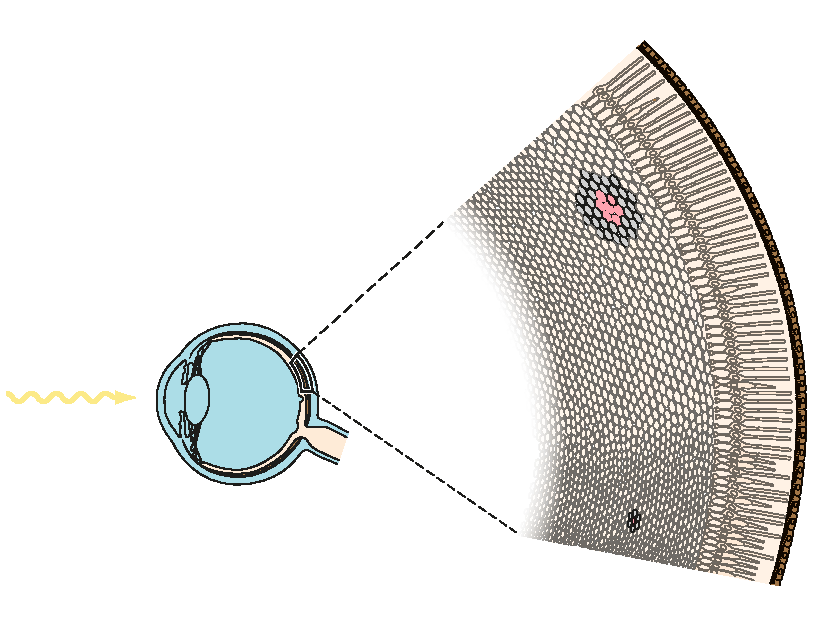
\includegraphics[width=0.8\textwidth]{assets/images/receptive-field.pdf}};
        
        % light
        \node[] (light) at (0.06\textwidth, 0.25\textwidth) {light};
        
        %cornea
        \node[] (corneatxt) at (0.15\textwidth, 0.37\textwidth) {cornea};
        \node[] (cornea) at (0.16\textwidth, 0.224\textwidth) {};
        \path [shadowarrow] (corneatxt) edge[bend right=10] node {} (cornea);
        \path [mainarrow] (corneatxt) edge[bend right=10] node {} ($ (cornea) + (-0.05, 0.2) $);
        
        %lens
        \node[] (lenstxt) at (0.2\textwidth, 0.33\textwidth) {lens};
        \node[] (lens) at (0.188\textwidth, 0.205\textwidth) {};
        \path [shadowarrow] (lenstxt) edge[bend right=7] node {} (lens);
        \path [mainarrow] (lenstxt) edge[bend right=7] node {} ($ (lens) + (-0.005, 0.2) $);
        
        % retina
        \node[] (retinatxt) at (0.33\textwidth, 0.35\textwidth) {retina};
        \node[] (retina) at (0.25\textwidth, 0.26\textwidth) {};
        \path [shadowarrow] (retinatxt) edge[bend left=7] node {} (retina);
        \path [mainarrow] (retinatxt) edge[bend left=7] node {} ($ (retina) + (0.19, 0.17) $);
        
        % fovea
        \node[] (foveatxt) at (0.4\textwidth, 0.25\textwidth) {fovea};
        \node[] (fovea) at (0.283\textwidth, 0.216\textwidth) {};
        \path [shadowarrow] (foveatxt) edge[bend left=7] node {} (fovea);
        \path [mainarrow] (foveatxt) edge[bend left=7] node {} ($ (fovea) + (0.2, 0.025) $);
        
        % receptive field
        \node[text width=0.8in] (RFperiphery) at (0.8\textwidth, 0.5\textwidth) {RF in the periphery};
        \node[text width=0.8in] (RFfovea) at (0.87\textwidth, 0.1\textwidth) {RF near the fovea};
        
    \end{scope}
\end{tikzpicture}
    \caption{Visual system and size variability of receptive fields (RF) depending on their eccentricity \cite{KandelBook2003:25}.}
    \label{fig:receptive-field}
\end{figure}

The segregation of figures from the background is an integral part of object recognition \cite{KandelBook2003:25}. The visual scenes are analyzed at three levels. At the low level, the discrimination on such visual attributes as local contrast, orientation, color, and movement occurs. The intermediate level is responsible for parsing an image into surfaces, their depths, shapes, and global contours and distinguishing foreground from background. Then, finally, at the highest level of visual analysis, object identification takes place.

\todo{I thought this entire work focuses on the low level, but it says that the segregation of figures from background happens at intermediate level?}

\paragraph{Receptive field}

The receptive field of a fiber is the area on the retina that responds to the light cast on this particular fiber. The receptive fields in the visual cortex perform the parsing of information from complex scenes into contours of individual objects and separate those from their background. Its size is measured in degrees of a visual angle, the entirety of which is nearly equal to $180^\circ$.
The central region of the retina, the fovea, corresponds to the center of the gaze and thus has the highest density of photoreceptors, leading to the greatest visual acuity. Eccentricity is defined as the distance between the receptive field center and fovea. Therefore, as depicted in Figure \ref{fig:receptive-field}, the number of photoreceptors in the receptive field receiving input is smaller when eccentricity is smaller, that is, the closer they are to the fovea.

The neurons' receptive fields follow a center-surround organization and have two functionally distinct subareas: on-center and off-center (pink and grey areas in Figure \ref{fig:receptive-field}, respectively). As depicted in Table \ref{tab:on-off-center}, the firing response of on- and off-center cells varies depending on the light location: the regions of the spatial contrast are emphasized, while little response is received from homogeneous illumination. The center and surrounding areas are mutually inhibitory, making the receptive field sensitive to borders and contours and thus allowing it to encode information about contrast.

\begin{table}[!htp]
    \centering
    \begin{tabular}{m{3cm}|c|c|c|}
\cline{3-4}
\multicolumn{2}{l|}{}                                                                  & \cellcolor{main-color}\textbf{on-center} & \cellcolor{main-color}\textbf{off-center} \\ \hline
\multicolumn{1}{|m{3cm}|}{\cellcolor{main-color}\textbf{\makecell{Light on \\ center only}}}   & \raisebox{-.5\height}{\begin{tikzpicture}
    \begin{scope}
        % to take up space
        \draw[draw=white, fill=white] (0, 0) circle (1.7cm);
        
        % off-center area
        \draw[dashed, draw=black, fill=gray-color] (0, 0) circle (1.5cm);
        % on-center area
        \draw[dashed, draw=black, fill=sec-color] (0, 0) circle (0.6cm);
        
        % light
        \draw[draw=main-color , fill=main-color] (0, 0) circle (0.3cm);
    \end{scope}
\end{tikzpicture}} & rapid firing                               & no firing                                   \\ \hline
\multicolumn{1}{|m{3cm}|}{\cellcolor{main-color}\textbf{\makecell{Light on \\ surround only}}} & \raisebox{-.5\height}{\begin{tikzpicture}
    \begin{scope}
        % to take up space
        \draw[draw=white, fill=white] (0, 0) circle (1.7cm);
        
        % off-center area
        \draw[dashed, draw=black, fill=gray-color] (0, 0) circle (1.5cm);
        % on-center area
        \draw[dashed, draw=black, fill=sec-color] (0, 0) circle (0.6cm);
        
        % light
        \draw[draw=main-color , fill=main-color] (1.05, 0) circle (0.3cm);
    \end{scope}
\end{tikzpicture}} & no firing                                  & rapid firing                                \\ \hline
\multicolumn{1}{|m{3cm}|}{\cellcolor{main-color}\textbf{\makecell{No light \\ on either}}}               & \raisebox{-.5\height}{\begin{tikzpicture}
    \begin{scope}
        % to take up space
        \draw[draw=white, fill=white] (0, 0) circle (1.7cm);
        
        % off-center area
        \draw[dashed, draw=black, fill=gray-color] (0, 0) circle (1.5cm);
        % on-center area
        \draw[dashed, draw=black, fill=sec-color] (0, 0) circle (0.6cm);
    \end{scope}
\end{tikzpicture}} & no firing                                  & no firing                                   \\ \hline
\multicolumn{1}{|m{3cm}|}{\cellcolor{main-color}\textbf{\makecell{Light on \\ both}}}          & \raisebox{-.5\height}{\begin{tikzpicture}
    \begin{scope}
        % to take up space
        \draw[draw=white, fill=white] (0, 0) circle (1.7cm);
        
        % off-center area + light
        \draw[dashed, draw=black, fill=main-color] (0, 0) circle (1.5cm);
        % on-center area + light
        \draw[dashed, draw=black, fill=main-color] (0, 0) circle (0.6cm);
    \end{scope}
\end{tikzpicture}} & mild/no firing                             & mild/no firing                              \\ \hline
\multicolumn{1}{|m{3cm}|}{\cellcolor{main-color}\textbf{\makecell{Light-dark \\ boundary}}}    & \raisebox{-.5\height}{\begin{tikzpicture}
    \begin{scope}
        % to take up space
        \draw[draw=white, fill=white] (0, 0) circle (1.7cm);
        
        % off-center area
        \draw[dashed, draw=black, fill=gray-color] (0, 0) circle (1.5cm);
        % on-center area
        \draw[dashed, draw=black, fill=sec-color] (0, 0) circle (0.6cm);
        
        % light
        \draw[draw=main-color, fill=main-color] (0.6cm, {1.5*sin(66.42)}) arc(66.42:293.58:1.5);
        
        % dashed on top
        \draw[dashed, draw=black] (0, 0) circle (0.6cm);
        \draw[dashed, draw=black] (0, 0) circle (1.5cm);
        
        
    \end{scope}
\end{tikzpicture}} & brisk firing                               & brisk firing                                \\ \hline
\end{tabular}
    \caption{Response of on- and off-center neurons depending on presence and location of light (yellow) in the receptive field \cite{KandelBook2003:25}.}
    \label{tab:on-off-center}
\end{table}

\paragraph{Grating stimuli}

Evidently, small spots of light are helpful for studying receptive fields of single neurons. However, in order to learn about visual perception, more complex stimuli are needed \cite{KandelBook2003:26}. For instance, grating stimuli are used to investigate the perception of spatial patterns. Such stimuli comprise images, where the luminosity varies about the mean as a sinusoidal function of space, as displayed in Figure \ref{fig:grating-stimuli-examples}. 

\begin{figure}[!htp]
    \centering
    \begin{subfigure}[t]{0.3\textwidth}
        \centering
        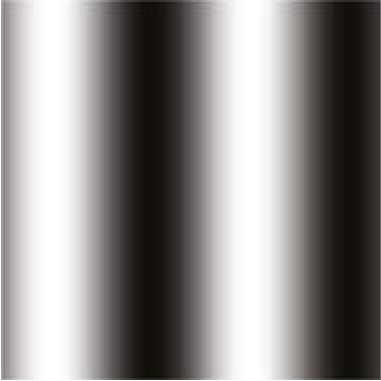
\includegraphics[width=0.65\textwidth]{assets/images/grating-stimuli/1.png}
        \caption{{Low spatial frequency.}}
    \end{subfigure}
    \hspace{0.03\textwidth}
    \begin{subfigure}[t]{0.3\textwidth}
        \centering
        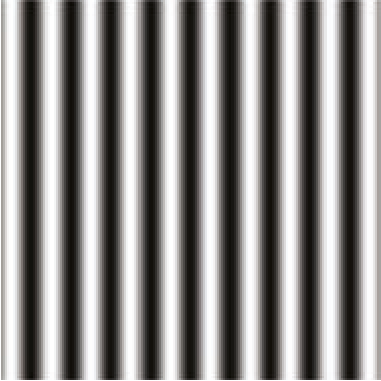
\includegraphics[width=0.65\textwidth]{assets/images/grating-stimuli/2.png}
        \caption{High spatial frequency, high contrast.}
    \end{subfigure}
    \hspace{0.03\textwidth}
    \begin{subfigure}[t]{0.3\textwidth}
        \centering
        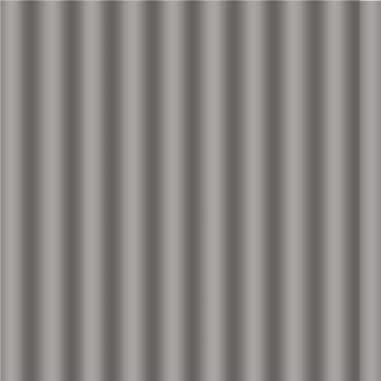
\includegraphics[width=0.65\textwidth]{assets/images/grating-stimuli/3.png}
        \caption{High spatial frequency, low contrast.}
    \end{subfigure}
    \caption{Examples of grating stimuli \cite{KandelBook2003:26}.}
    \label{fig:grating-stimuli-examples}
\end{figure}
